\graphicspath{ {./root/4.Annex/3.AnnexLorenzoInspectionImages/} }

\subsection{Evaluator 3 inspection scores}

\begingroup
\setlength{\tabcolsep}{1.5cm}
\renewcommand{\arraystretch}{1.45}

\rowcolors{2}{lightgray}{lightblue}
\begin{longtable}{l r}
	
	\hiderowcolors
	\textbf{Heuristic} & \textbf{Score} \\ \hline  \endhead \\
	\showrowcolors
	
	H1. Visibility of system status & 2  \\
	H2. Match between system and the real world & 4  \\
	H3. User control and freedom & 2 \\
	H4. Consistency and standards & 3 \\
	H5. Error prevention & 4 \\
	H6. Recognition rather than recall & 5 \\
	H7. Flexibility and efficiency of use & 3 \\
	H8. Aesthetic and minimalist design & 2 \\
	H9. Help users recognize, diagnose and recover from errors & 4 \\
	H10. Help and documentation & 3 \\
	H11. Information overload & 2 \\
	H12. Consistency of page content structure  & 3 \\
	H13. Contextualized information & 2 \\
	H14. Content organization (hierarchy) & 5 \\
	H15. Interaction consistency & 2 \\
	H16. Group navigation-1 & 2 \\
	H17. Group navigation-2 & 5 \\
	H18. Structural navigation & 4 \\
	H19. Semantic navigation & 3 \\
	H20. “Landmarks” & 4 \\
	H21. Text lay out & 4 \\
	H22. Interaction placeholders-semiotics & 5 \\
	H23. Interaction placeholders-consistency & 2 \\
	H24. Consistency of visual elements & 3 \\
	H25. Hierarchy-1 & 4 \\
	H26. Hierarchy-2 & 3 \\
	H27. Spatial allocation-1 & 5 \\
	H28. Spatial allocation-2 & 5 \\
	H29. Consistency of page spatial structure & 4 \\
	
\end{longtable}

\endgroup

\clearpage

\subsection*{Evaluator's comments}
\paragraph*{H1. Visibility of System Status – Score 2}
The orientation information in general is not very useful or clear. Indeed, there are few instances where there are helpful breadcrumbs:
\begin{itemize}
	\item \textit{\href{https://www.unicef.org/protection/child-marriage}{UNICEF - Child Marriage}}
	\item \textit{\href{https://www.unicef.org/gender-equality}{UNICEF - Gender Equality}}
	\item \textit{\href{https://www.unicef.org/immunization/polio}{UNICEF - Polio Immunization}}
\end{itemize}

In general, there is interactive orientation information almost exclusively in the “What we do” section. In fact, in other parts of the site in which breadcrumbs would have been useful, they are absent like in the “Stories” section (e.g., \textit{\href{https://www.unicef.org/emergencies/13-emergencies-need-more-attention-support-2024}{UNICEF - Emergencies}}) or in the “About us” section (e.g., \textit{\href{https://www.unicef.org/about-us/75-years-unicef}{UNICEF - About Us}}).
However, even among the present ones there are various inconsistencies in the depth and thought behind them. In addition, the “Home” label is redundant, due to the constant presence of the UNICEF logo in the top left corner.\\
The breadcrumbs show the user where they are in the website’s hierarchy and not their own path that led them to that page, so they are not dynamically generated (e.g., from \textit{\href{https://www.unicef.org/gender-equality}{UNICEF - Gender Equality}} to \textit{\href{https://www.unicef.org/protection/child-marriage}{UNICEF - Child Marriage}}).

\begin{figure}[h]
	
\includegraphics[width=\textwidth]{Picture1.png}
	\captionsetup{font=small}
	\caption{\textit{Breadcrumb example.}}
	\label{fig:label1}
\end{figure}

\paragraph*{H2. Match Between the System and the Real World – Score 4}
The site presents easily understandable language, even in more specialized and delicate topics, it utilizes specific words consciously, and the articles' contents are generally easy to read.
Example: \textit{\href{https://www.unicef.org/gender-equality}{UNICEF - Gender Equality}}

In addition, there are clear and comprehensible icons about the main topics of the website.
Example: \textit{\href{https://www.unicef.org/}{UNICEF Homepage}}

However, there are instances where the adopted solutions are not as clear as they could have been, like on the page: \textit{\href{https://www.unicef.org/where-we-work}{UNICEF - Where We Work}}. The “Browse areas by alphabetical listing” is understandable enough, but it would have been much better with a graphical representation of a map where users could click on the particular nation.
\begin{figure}[h]
	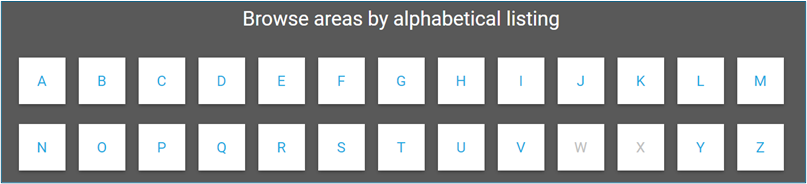
\includegraphics[width=\textwidth]{Picture3.png}
	\captionsetup{font=small}
	\caption{\textit{Browse areas by alphabetical listing.}}
	\label{fig:label2}
\end{figure}
\begin{figure}[h]
	\centering
	\begin{center}
		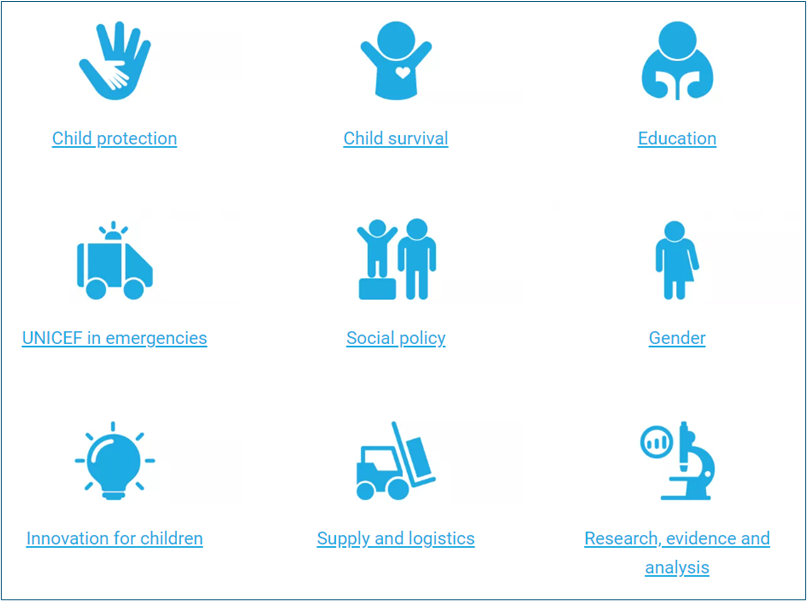
\includegraphics[width=0.6\textwidth]{Picture2.png}
	\end{center}
	\captionsetup{font=small}
	\caption{\textit{Icons example on the homepage.}}
	\label{fig:label3}
\end{figure}


\paragraph*{H3. User Control and Freedom – Score 2}
If you miss click on a link there is no way to go back apart from the browser back arrow, since there is no use of capillary breadcrumbs and no other method of navigation on the website. So, the user can only go forward in their path, while the opposite is not really implemented.
It is also fair to say, however, that there are not many functionalities that actually need to implement undo and redo actions, since the website is informative and lets the user do almost nothing apart from reading and navigation. The only notable example is the donate page.

\paragraph*{H4. Consistency and Standars – Score 3}
The website is mostly consistent in its appearance, use of colours, fonts, and in general standards. However, there are some major instances that violate this principle:
\begin{itemize}
	\item Different websites and layout depending on the language (e.g., \href{https://www.unicef.org/es}{UNICEF Spanish Website})
	\begin{figure}[h]
		
\includegraphics[width=\textwidth]{Picture4.png}
		\captionsetup{font=small}
		\caption{\textit{ES Header.}}
		\label{fig:label4}
	\end{figure}
	\item Different actions when interacting with the label of the drop-down menus: clicking on “What we do” will bring the user to \href{https://www.unicef.org/what-we-do}{UNICEF - What We Do}, which is the first focus area “All areas”, while clicking on “Research and reports” will bring the user to a completely new and non-reachable page through the sub labels \href{https://www.unicef.org/research-and-reports}{UNICEF - Research and Reports}.
	\item Different and ambiguous meaning, labeling, and colours for different cards throughout the website. They are clearly dependent on the type of information, but not in a consistent way. Sometimes they are white for different types of cards, then some are blue for the same type (maybe more important), most have images but some do not, there are rare black ones that seem out of place.
\end{itemize}
\begin{itemize}
	\item \href{https://www.unicef.org/reports/adolescent-girls-programme-strategy-2022-2025}{UNICEF - Adolescent Girls Programme Strategy 2022-2025}
	\begin{figure}[h]
		\centering
		\begin{center}
			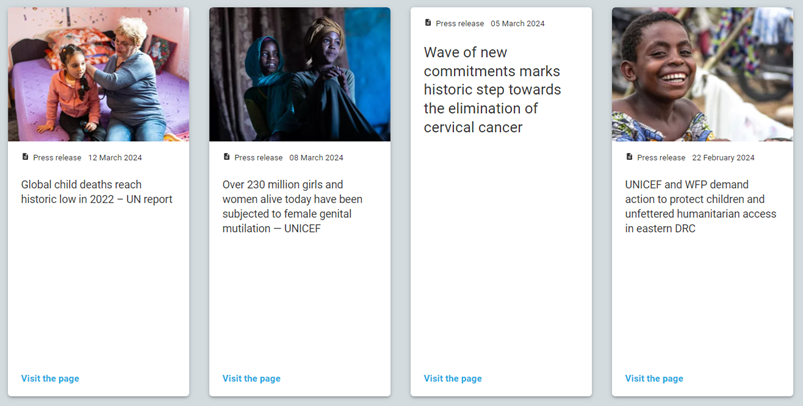
\includegraphics[width=0.6\textwidth]{Picture5.png}
		\end{center}
		\captionsetup{font=small}
		\caption{\textit{Card inconsistency example 1.}}
		\label{fig:label5}
	\end{figure}
	\item \href{https://www.unicef.org/partnerships/public}{UNICEF - Partnerships}
	\begin{figure}[h]
		\centering
		\begin{center}
			
\includegraphics[width=0.6\textwidth]{Picture6.png}
		\end{center}
		\captionsetup{font=small}
		\caption{\textit{Card inconsistency example 2.}}
		\label{fig:label6}
	\end{figure}
	\item \href{https://www.unicef.org/gender-equality/skills4girls}{UNICEF - Skills4Girls}
	\begin{figure}[h]
		\centering
		\begin{center}
			
\includegraphics[width=0.6\textwidth]{Picture7.png}
		\end{center}
		\captionsetup{font=small}
		\caption{\textit{Card inconsistency example 3.}}
		\label{fig:label7}
	\end{figure}
\end{itemize}

\newpage

\paragraph*{H5. Error Prevention – Score 4}
There are not many instances of possible error-prone actions.
However, in the donation page (\href{https://donazioni.unicef.it/}{UNICEF Donation Page}), which is one of the few pages in which the user can actually interact with the site, when filling out the form there is no double check for the user email or a pop-up to encourage the user to check again their data for both personal and bank/card information. This should be done since it is a delicate and sensitive step where money is involved.
\begin{figure}[h]
	\centering
	\begin{center}
		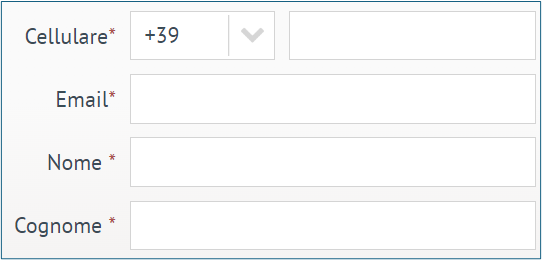
\includegraphics[width=0.6\textwidth]{Picture8.png}
	\end{center}
	\captionsetup{font=small}
	\caption{\textit{Donation form - Personal information.}}
	\label{fig:label8}
\end{figure}
\begin{figure}[h]
	\centering
	\begin{center}
		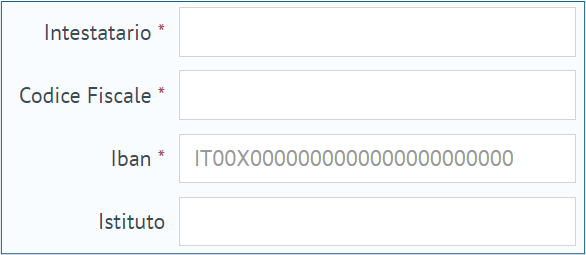
\includegraphics[width=0.6\textwidth]{Picture9.png}
	\end{center}
	\captionsetup{font=small}
	\caption{\textit{Donation form - Banking information.}}
	\label{fig:label9}
\end{figure}

\newpage

\paragraph*{H6. Recognition rather than Recall – Score 5}
All needed information is readily available on the page; for example, all articles are self-contained and do not spill into other pages, forcing the user to remember information from one page to another. General information is easily retrievable via sections and labels, and for more in-depth information, there is the section about reports (e.g., \href{https://www.unicef.org/reports/state-of-worlds-children}{UNICEF - State of the World's Children}) and to search for a particular topic, article, or data there is the website \href{https://data.unicef.org/}{UNICEF Data}, accessible via the link “Data by topic and country” in the “Research and reports” section.
\begin{figure}[h]
	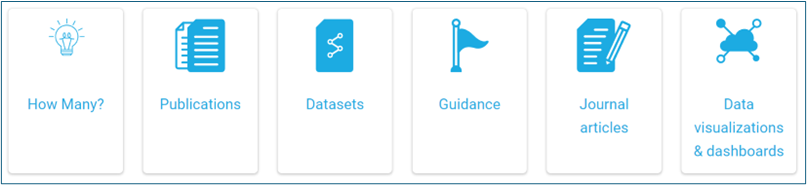
\includegraphics[width=\textwidth]{Picture10.png}
	\captionsetup{font=small}
	\caption{\textit{Data UNICEF catalog of options.}}
	\label{fig:label10}
\end{figure}

\paragraph*{H7. Flexibility and Efficiency of Use – Score 3}
The website does not present any particular outstanding example of web accelerators. There are various sections, but the only accelerators are the donate button and the press centre one. The first brings the user to the donate page of UNICEF (\href{https://donazioni.unicef.it/}{UNICEF Donation Page}), which is probably one of their main goals with the website (but it is not a recurrent action for a normal or advanced user). While the latter brings the user to the latest news of UNICEF (\href{https://www.unicef.org/media/press-centre}{UNICEF - Press Centre}), which might be more useful for the advanced user, since this might be an action frequently executed and that cuts the user’s time to find the latest news.
\begin{figure}[h]
	\centering
	\begin{center}
		
\includegraphics[width=0.6\textwidth]{Picture11.png}
	\end{center}
	\captionsetup{font=small}
	\caption{\textit{Data UNICEF catalog of options.}}
	\label{fig:label11}
\end{figure}

\paragraph*{H8. Aesthetic and Minimalist Design – Score 2}
The site, in general, is very over saturated with information, different sections, images, cards, links, icons, drop-down menus, and so on. Some pages, like the home page (\href{https://www.unicef.org/}{UNICEF Homepage}), are still acceptable. On the home page, there are many things distracting the user, but there is some space between them, and the cards and icons help unclutter a bit the page. Another good page is the donate page (\href{https://donazioni.unicef.it/}{UNICEF Donation Page}).\\
On the contrary, many pages like \href{https://www.unicef.org/gender-equality/skills4girls}{UNICEF - Skills4Girls}, or \href{https://www.unicef.org/reports/state-worlds-children-2023#SOWC}{UNICEF - State of the World's Children 2023} are filled with a lot of different information and in various formats, with abundant links and photos, creating very long and difficult to absorb pages.
\begin{figure}[h]
	\centering
	\begin{center}
		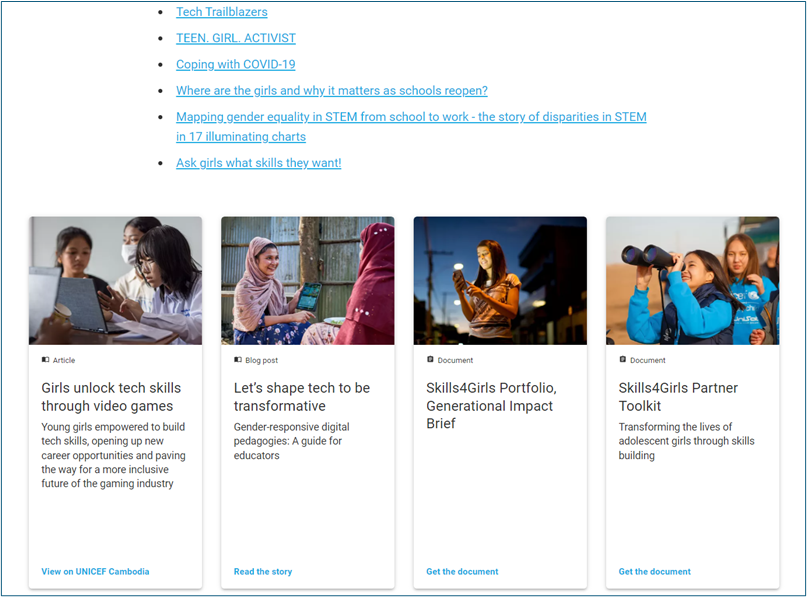
\includegraphics[width=0.52\textwidth]{Picture12.png}
	\end{center}
	\captionsetup{font=small}
	\caption{\textit{Example of the many possibilities of interaction for an user in a small space.}}
	\label{fig:label12}
\end{figure}

\paragraph*{H9. Help Users Recognize, Diagnose and Recover from Error – Score 4}
There is a broken link on the page \href{https://www.unicef.org/partnerships}{UNICEF - Partnerships} when clicking on the JOIN UNICEF button. There is a clear back button to recover from the error, but the error message itself is quite generic. In addition, it should be a quite important page, since it is among the ones letting you start your journey with UNICEF.
\begin{figure}[h]
	\centering
	\begin{center}
		
\includegraphics[width=0.5\textwidth]{Picture13.png}
	\end{center}
	\captionsetup{font=small}
	\caption{\textit{Error message.}}
	\label{fig:label13}
\end{figure}
\\
In the donation page (\href{https://donazioni.unicef.it/}{UNICEF Donation Page}), there are clear and minimal messages about what is the problem with each field of the donor.
\begin{figure}[h]
	\centering
	\begin{center}
		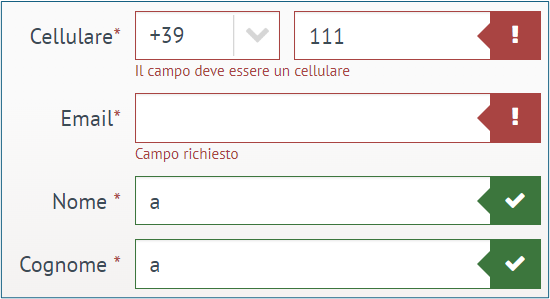
\includegraphics[width=0.6\textwidth]{Picture14.png}
	\end{center}
	\captionsetup{font=small}
	\caption{\textit{Error messages.}}
	\label{fig:label14}
\end{figure}

\newpage

\paragraph*{H10. Help and Documentation – Score 3}
The website is straightforward to use, navigate, and perform actions on. In addition, there are Frequently Asked Questions in their own dedicated page (\href{https://www.unicef.org/about-unicef/frequently-asked-questions}{UNICEF - Frequently Asked Questions}), accessible via link in the footer of the page. The page is not particularly rich and the last question: “I am having difficulty finding specific information on UNICEF.org. Where should I go?” is not really answered to help the user. In fact, it could have been much better if there was at least a link to other UNICEF related websites or the website \href{https://data.unicef.org/}{UNICEF Data}.

\paragraph*{H11. Information Overload – Score 2}
The site, in general, is very over saturated with information, different sections, images, cards, links, icons, drop-down menus, and so on.
Some pages, like the home page (\href{https://www.unicef.org/}{UNICEF Homepage} or \href{https://www.unicef.org/gender-equality}{UNICEF - Gender Equality}), are still acceptable. In these pages, there are many things for the user, but there is some space between them, and cards and icons help unclutter the page, aiding in organizing and making the content more readable. Another good page is the donate page (\href{https://donazioni.unicef.it/}{UNICEF Donation Page}).\\
On the contrary, many pages like \href{https://www.unicef.org/gender-equality/skills4girls}{UNICEF - Skills4Girls} are filled with a lot of different information and in various formats, with abundant links and photos, creating very long and difficult to absorb pages.\\
Another example is \href{https://www.unicef.org/reports/global-annual-results-2021-gender-equality}{UNICEF - Global Annual Results 2021 Gender Equality}, where the drop-down menus help organize and clean the page (even though there are 11 of them), but then there are 7 little links all together in a very small area.
\begin{figure}[h]
	\centering
	\begin{center}
		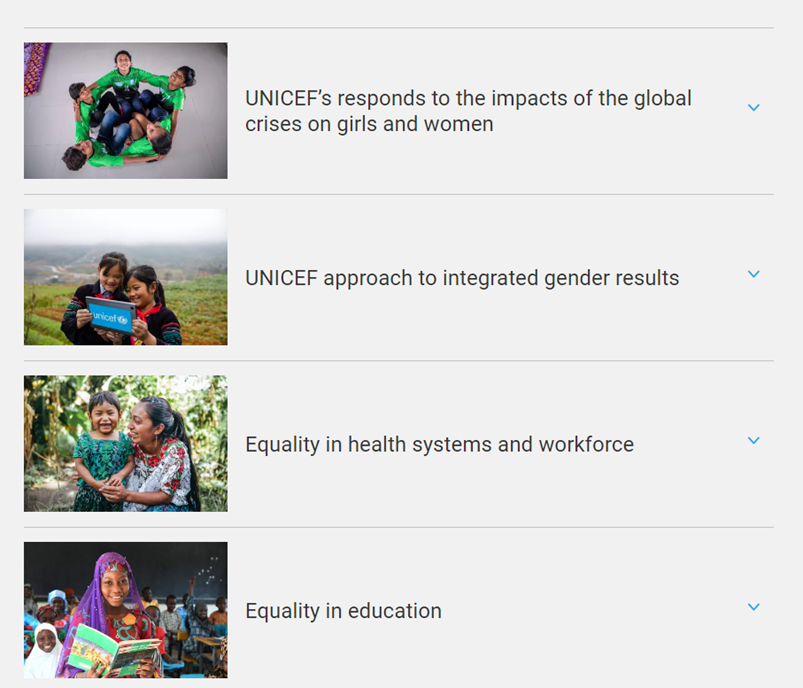
\includegraphics[width=0.6\textwidth]{Picture15.png}
	\end{center}
	\captionsetup{font=small}
	\caption{\textit{Example drop-down menu.}}
	\label{fig:label15}
\end{figure}
\begin{figure}[h]
	\centering
	\begin{center}
		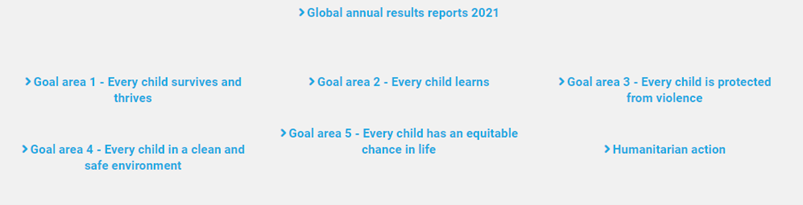
\includegraphics[width=0.7\textwidth]{Picture16.png}
	\end{center}
	\captionsetup{font=small}
	\caption{\textit{Example small links.}}
	\label{fig:label16}
\end{figure}

\newpage

\paragraph*{H12. Consistency of Page Content Structure – Score 3}
The site presents content of the same type in a similar fashion most of the time, even though there are also many instances of inconsistencies.
Pages examined: \href{https://www.unicef.org/gender-equality}{UNICEF - Gender Equality} and \href{https://www.unicef.org/health}{UNICEF - Health}. They are both pages of the section “What we do” and they represent a good consistency example. In addition, cards of the same type (“Article”, “Report”, “Blog Post”, etc.) share the exact same style and structure making them very consistent.
However, in the smaller details also pages of the same type present differences like in the two “Appeal” pages: \href{https://www.unicef.org/emergencies/emergency-response-sudan}{UNICEF - Emergency Response Sudan} and \href{https://www.unicef.org/emergencies/crisis-haiti}{UNICEF - Crisis Haiti}.
\begin{figure}[h]
	\centering
	\begin{center}
		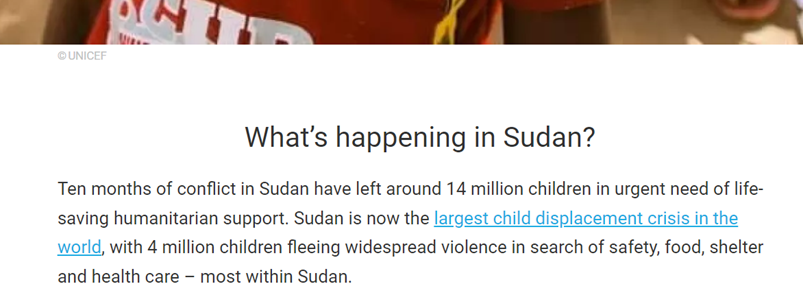
\includegraphics[width=0.7\textwidth]{Picture17.png}
	\end{center}
	\captionsetup{font=small}
	\caption{\textit{Difference in the header of articles of the same kind.}}
	\label{fig:label17}
\end{figure}
\begin{figure}[h]
	\centering
	\begin{center}
		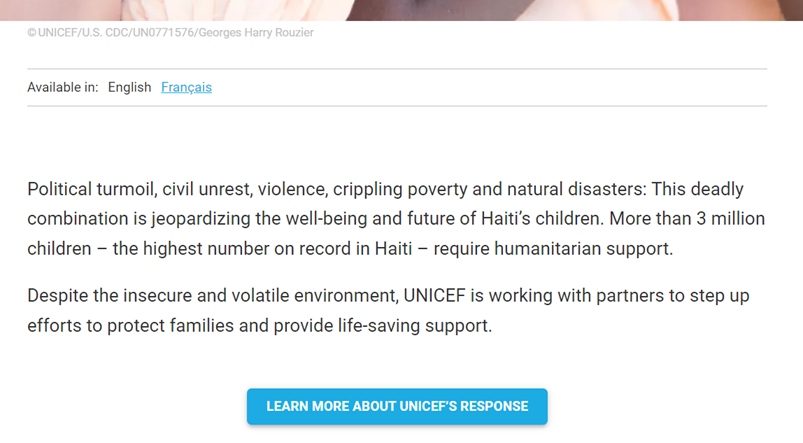
\includegraphics[width=0.7\textwidth]{Picture18.png}
	\end{center}
	\captionsetup{font=small}
	\caption{\textit{Difference in the header of articles of the same kind.}}
	\label{fig:label18}
\end{figure}

\paragraph*{H13. Contextualized Information – Score 2}
Similar motivations to H1.\\
The website offers the user some breadcrumbs and hints (like URL) to tell where they are, but they are not enough, not pervasive enough, and on some occasions misleading. Furthermore, some links lead to entirely different UNICEF websites.

\paragraph*{H14. Content Organisation (Hierarchy) – Score 5}
The content is organized in an understandable manner, it is not the most intuitive, but it has its meaning. In hierarchical sense the different pages are mostly well organized:
\begin{itemize}
	\item Via the main 5 sections
	\item Via the subsections
	\item Via hierarchical relations inside pages (e.g., \href{https://www.unicef.org/gender-equality/skills4girls}{UNICEF - Skills4Girls})
\end{itemize}
The sections and categories are well organized, but sometimes they are redundant in the hierarchy, since they may belong to various sections like \href{https://www.unicef.org/partnerships}{UNICEF - Partnerships} which belongs both to “Take action” and “What we do”, even though it could have been present in only the first instance.

\paragraph*{H15. Interaction Consistency – Score 2}
In the most general sense, the navigation in pages of the same type is somewhat consistent. However, there are instances in which this is not the case:
\begin{itemize}
	\item Different actions when interacting with the label of the drop-down menus: clicking on “What we do” will bring the user to \href{https://www.unicef.org/what-we-do}{UNICEF - What we do}, which is the first focus area “All areas”, while clicking on “Research and reports” will bring the user to a completely new and non-reachable page through the sub labels \href{https://www.unicef.org/research-and-reports}{UNICEF - Research and Reports}
	\item On the home page clicking on the icons does not bring the user directly to that page, but to a section below which subsequently leads to the wanted page.
	\item Clicking on the label “Central African Republic” brings to a completely different page: \href{https://www.unicef.org/car/en}{UNICEF - Central African Republic}
	\item On a page level, even on similar pages, like \href{https://www.unicef.org/immunization}{UNICEF - Immunization} and \href{https://www.unicef.org/gender-equality}{UNICEF - Gender Equality} which are both pages of the section “What we do”, there are similarities but there are also many differences about how the user can interact, for example one has drop-down menu and the other does not.
\end{itemize}

\paragraph*{H16. Group Navigation 1 – Score 2}
It is easy to navigate from the general section to sub-pages, but not the other way around (only back arrow of browser) and not even among those sub-pages. For example: from a page it is easy to visit its related articles, but it is difficult to go back. Moreover, it is not the best experience to navigate among them, since there are article cards at the end of the page, but they may not be the same as before.
\begin{itemize}
	\item From \href{https://www.unicef.org/gender-equality}{UNICEF - Gender Equality} to \href{https://www.unicef.org/blog/why-i-champion-gender-equity}{UNICEF Blog: Why I Champion Gender Equity}
	\begin{figure}[h]
		\centering
		\begin{center}
			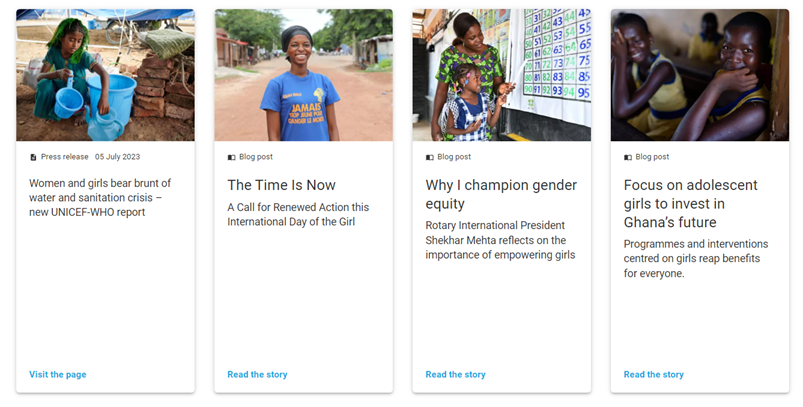
\includegraphics[width=0.6\textwidth]{Picture19.png}
		\end{center}
		\captionsetup{font=small}
		\caption{\textit{Example set of cards.}}
		\label{fig:label19}
	\end{figure}
	\item From \href{https://www.unicef.org/blog/why-i-champion-gender-equity}{UNICEF Blog: Why I Champion Gender Equity}, there are different cards.
	\begin{figure}[h]
		\centering
		\begin{center}
			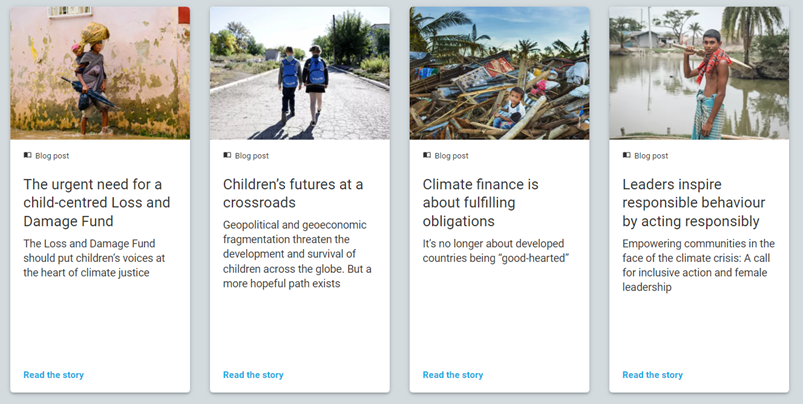
\includegraphics[width=0.6\textwidth]{Picture20.png}
		\end{center}
		\captionsetup{font=small}
		\caption{\textit{Example set of cards.}}
		\label{fig:label20}
	\end{figure}
	
\end{itemize}

\paragraph*{H17. Group Navigation 2 – Score 5}
Menus are rare in the website and where they are present, like in the top persistent navigation, in \href{https://www.unicef.org/where-we-work}{UNICEF - Where We Work} or in \href{https://data.unicef.org/resources/resource-type/publications/}{UNICEF Data - Publications}, they are clear and well done, presenting information in a non-intrusive or overloading manner.

\paragraph*{H18. Structural Navigation – Score 4}
Most of the time, navigating through a page topic is easy and pleasant, but there are some instances where navigating among the different parts of a topic is cumbersome due to long scrolls through moving background images (e.g., \href{https://www.unicef.org/reports/state-worlds-children-2023#SOWC}{UNICEF - State of the World's Children 2023}).\\ Navigating through different parts of a topic across pages is quite easy since there are many useful branching links, but going back to continue on the previous page is not.

\paragraph*{H19. Semantic Navigation – Score 3}
It is usually easy to navigate from one topic to another, but not vice versa. The only instances in which this is not true, and the navigation is bi-directional and easy are:
\begin{itemize}
	\item Between pages that are indexed in the sections/sub-sections of the top drop-down bar;
	\item Or between pages that have correct breadcrumbs (e.g., \href{https://www.unicef.org/protection/gender-based-violence-in-emergencies}{UNICEF - Gender-Based Violence in Emergencies}).
\end{itemize}
Because otherwise, there is always a forced directionality from the “parent” to the “child” page (e.g., \href{https://www.unicef.org/gender-equality}{UNICEF - Gender Equality} to \href{https://www.unicef.org/protection/gender-based-violence-in-emergencies}{UNICEF - Gender-Based Violence in Emergencies}).

\paragraph*{H20. Landmarks – Score 4}
Landmarks are useful to reach the most relevant pages, the main one is the home page UNICEF logo and in second the top drop-down bar. They are clear and bring the user to the starting pages of their possible searches for the various topics.\\
A not very helpful landmark is the “Donate” button, which is always present even though a typical user does not need it all the time (but it still has its meaning from the point of UNICEF business). While the press centre brings the user to the latest news of UNICEF (\href{https://www.unicef.org/media/press-centre}{UNICEF - Press Centre}), which might be more useful.\\
On the other side, some landmarks like the “high contrast” are not useful at all since not working properly.

\paragraph*{H21. Text Layout – Score 4}
The text is readable throughout the whole website. Font, size, and colour are appropriate for the situations presented on the website.
However, there are instances in which this is not respected, like in the page: \href{https://www.unicef.org/what-we-do}{UNICEF - What We Do} where the links are strikingly smaller than the rest.
\begin{figure}[h]
	\centering
	\begin{center}
		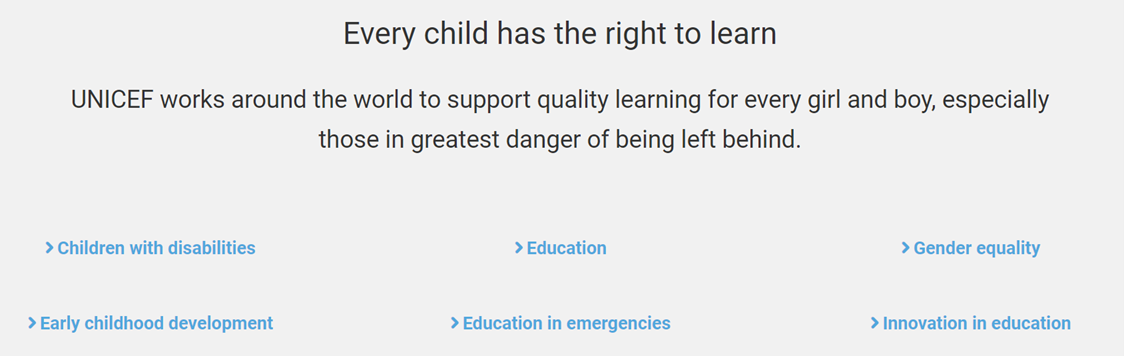
\includegraphics[width=0.7\textwidth]{Picture21.png}
	\end{center}
	\captionsetup{font=small}
	\caption{\textit{Example smaller links.}}
	\label{fig:label21}
\end{figure}

\paragraph*{H22. Interaction Placeholders - Semiotics – Score 5}
Interactive elements are very intuitive, easy to find, and use. Links in text format are clearly highlighted and intuitive, the same goes for icons, buttons, cards, and images.
\begin{figure}[h]
	\centering
	\begin{center}
		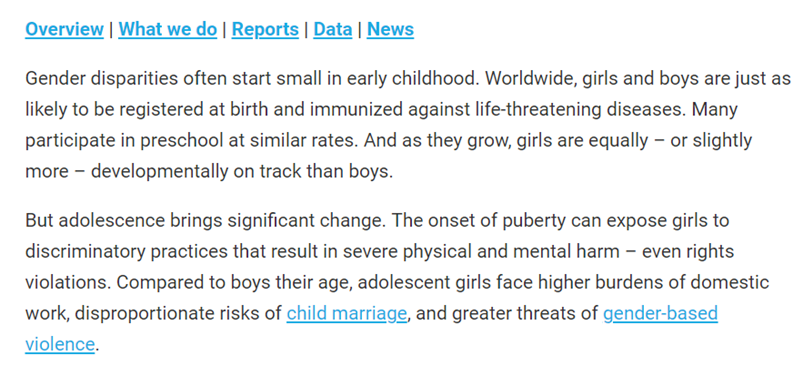
\includegraphics[width=0.7\textwidth]{Picture22.png}
	\end{center}
	\captionsetup{font=small}
	\caption{\textit{Example clearly visible interact-able links.}}
	\label{fig:label22}
\end{figure}
\\
The labels of the sections on the top drop-down bar are okay. The only non-intuitive aspect is the fact that the user can click on the main labels, like “What we do”, like a link, which brings them to another page instead of simply not doing anything or just dropping down the menu.

\paragraph*{H23. Interaction Placeholders - Consistency – Score 2}
There are some general instances where the textual and visual labels of interactive elements are consistent, but there are many more cases in which this property is not respected at all, like with the “Donate” button which can be found in different forms, and it is fundamental for the site.
\begin{figure}[h]
	
\includegraphics[width=\textwidth]{Picture23.jpg}
	\captionsetup{font=small}
	\caption{\textit{Example smaller links.}}
	\label{fig:label23}
\end{figure}
\\
Another instance of bad consistency is the cards for the various types of content (referencing H4). Also the placement of these elements is very different throughout the whole site.

\paragraph*{H24. Consistency of Visual Elements – Score 3}
The content is, in general, consistent in its visual department in pages of the same type (like \href{https://www.unicef.org/gender-equality}{UNICEF - Gender Equality} and \href{https://www.unicef.org/health}{UNICEF - Health}) like for the title, images, text position, etc., but still presents many inconsistencies, like the donate button, cards or icons.

\paragraph*{H25. Hierarchy 1 – Score 4}
The on-screen location of the various content is appropriate for their relevance, for the topic of the page and for the needs of the user.\\
For example, in \href{https://www.unicef.org/gender-equality}{UNICEF - Gender Equality}, the information is placed coherently and reflects the needs and wants of a user, following a logical and appropriate vertical order. However, there is not a clear hierarchical distinction among different parts regarding colours or title size.

\paragraph*{H26. Hierarchy 2 – Score 3}
The visual elements are in some cases well placed like buttons for donating, icons, and images on cards.\\
On other occasions like for images at the beginning of pages (e.g., \href{https://www.unicef.org/gender-equality}{UNICEF - Gender Equality}) are too big and not appropriate for their relevance.

\paragraph*{H27. Spatial Allocation 1 – Score 5}
Semantically related elements are grouped together quite well and appropriately on the website.
\begin{figure}[h]
	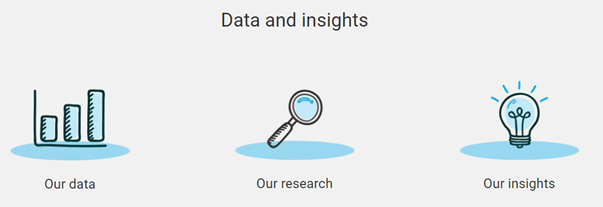
\includegraphics[width=\textwidth]{Picture24.png}
	\captionsetup{font=small}
	\caption{\textit{Example well grouped icons.}}
	\label{fig:label24}
\end{figure}
\begin{figure}[h]
	\centering
	\begin{center}
		
\includegraphics[width=0.6\textwidth]{Picture26.png}
	\end{center}
	\captionsetup{font=small}
	\caption{\textit{Example well grouped icons.}}
	\label{fig:label25}
\end{figure}
\begin{figure}[h]
	\centering
	\begin{center}
		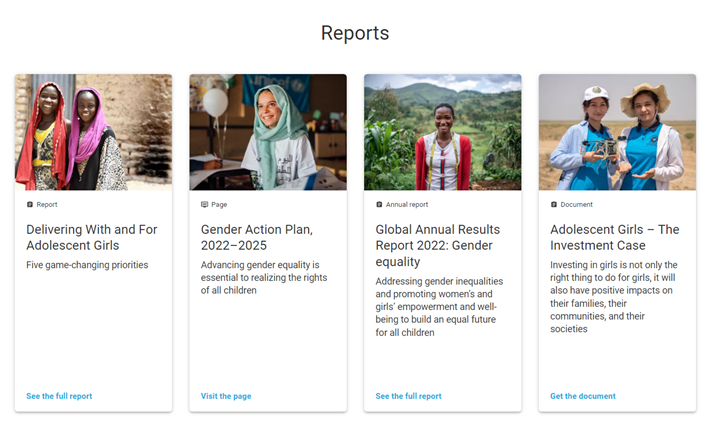
\includegraphics[width=0.6\textwidth]{Picture25.png}
	\end{center}
	\captionsetup{font=small}
	\caption{\textit{Example well grouped cards.}}
	\label{fig:label26}
\end{figure}

\paragraph*{H28. Spatial Allocation 2 – Score 5}
Semantically distant elements are usually placed far enough from each other to not cause confusion since they are separated into different sections of the website via colours and lines.
\begin{figure}[h]
	\centering
	\begin{center}
		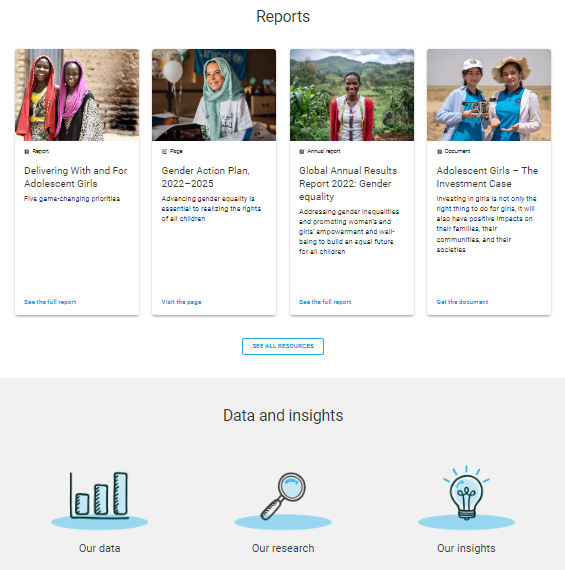
\includegraphics[width=0.7\textwidth]{Picture27.png}
	\end{center}
	\captionsetup{font=small}
	\caption{\textit{Example separation among different elements.}}
	\label{fig:label27}
\end{figure}

\newpage

\paragraph*{H29. Consistency of Page Spatial Structure – Score 4}
Pages of the same type share a similar spatial structure for their visual elements, this in general and most of the time.\\
But there are instances where pages of the same kind (e.g., \href{https://www.unicef.org/emergencies/delivering-support-afghanistans-children}{UNICEF - Delivering Support Afghanistan's Children} and \href{https://www.unicef.org/emergencies/children-gaza-need-lifesaving-support}{UNICEF - Children Gaza Need Lifesaving Support}) have different visual elements (not consistent): like buttons and videos, or completely different sections.
